\chapter{Model Development and Results}
\section{Results Magnetic Resonance}
We will discuss algorithmic approach on developing the generalized Kubo-Anderson model. We will describe general computational pitfalls that was faced during the software development and proposed solutions and tools to simulate stochastic behavior of the interacting systems in applied magnetic field. The introduction to Masters equation and transition rate matrix construction will be covered as well. At the end of the chapter we will cover Hamiltonian construction and difference between various models in low and high field approximations.
\subsection{Algorithm to find inverse of Liouville Matrix}\label{algorithmsection}
In order to obtain lineshape from stochastic approach on relaxation effects of spin dynamics it is important to asset proper inversion algorithm of Liouville matrix from Eq\.Ref{eq:35}. Liouville matrix can be represented as two dimensional array where each index of the dimension has and additional three sub-indexes specified by stochastic and electron or/and nuclus spin states. In other words: 
\begin{equation}\label{eq:53}
\mathcal{L}_{i,j}=\mathcal{L}_{a,m_0,m_1;b,m_0',m_1'}  
\end{equation}  
Where $i\rightarrow a,m_0,m_1$ and $j\rightarrow b,m_0',m_1'$. Computationally there are two distinctive approaches on populating and inverting the matrix. In the first approach Liouville matrix kept two dimensional and general rule on encoding each index into three sub-indexes should be elaborated. This task is ambiguous and probability of undiscovered omission while perfect compilation is high. From the second approach Liouville two dimensional matrix can be deployed into higher dimensions where each dimension is specified according to quantum and stochastic states:  
\begin{equation}\label{eq:54}
\mathcal{L}_{i,j}=\mathcal{L}_{a,m_0,m_1;b,m_0',m_1'}\rightarrow \mathcal{L}_{a,m_0,m_1,b,m_0',m_1'}
\end{equation}
The need of such transformation is to simplify assignment of Liouville matrix according to the action of spin operators on quantum states and tracking of stochastic states. Also it will simplify summation that have to be performed in order to compute line shape from Eq. 33. Access of matrix elements of dimensions higher than 2 can be illustrated through concept of the "page" representation on fig. 4. 
\begin{figure}[h!]
\centering
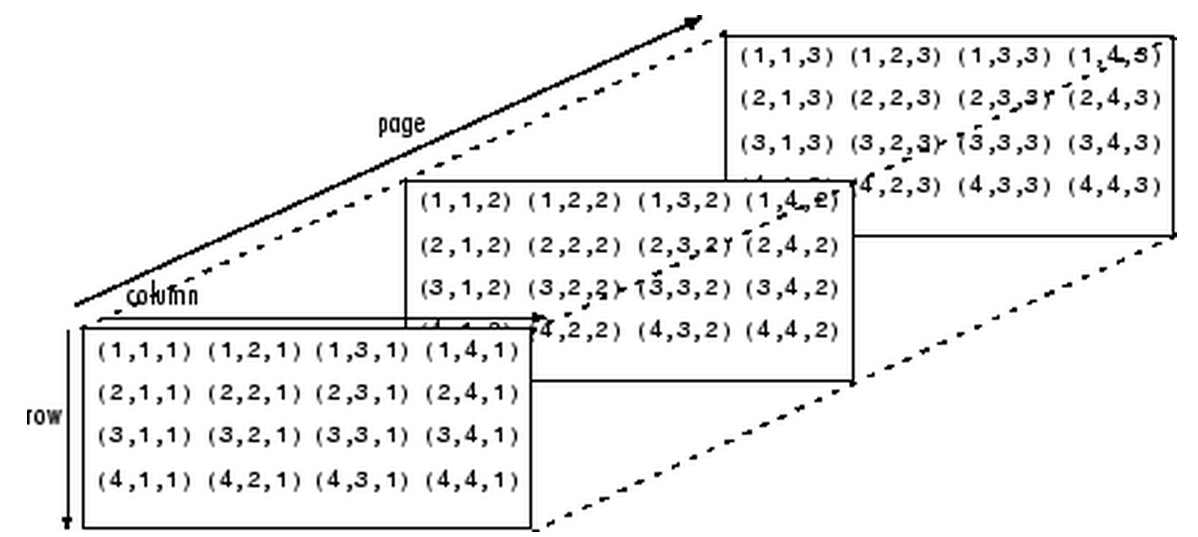
\includegraphics[width=0.7\textwidth]{figures/chap1/mat.png}
\caption{Illustration of "page" concept of storing and accessing elements of 3-dimensional array $A_{4,4,4}$ or $A[4,4,4]$ with four elements in each dimension.~\cite{Matlab}}
\end{figure}
\\
For example Liouville matrix for isolated nuclear spin has six dimensions $\Big(\mathcal{L}[a,m_0,m_1,b,m_0',m_1']\Big)$ and if electron spin interaction is added it expands to overall ten dimensions specified by four additional sub-indexes $m_{0S},m_{1S},m_{0S}',m_{1S}'$ or $\Big(\mathcal{L}[a,m_{0S},m_{1S},m_0,m_1,b,m_{0S}',m_{1S}',m_0',m_1']\Big)$. \\
Issue arises from the fact that matrix inversion of the multidimensional array is limited to finding inverse of every specified "page" rather then whole array structure. Transition from higher dimensions to dimension where it is possible to perform matrix inversion is important step in computational algorithm. While transforming from N-dimensions to two dimensions where matrix inverse can be found it is important to track the indexes transformation. In order to achieve proper index transformation a hash table should be created. \\*
 Example of hash table for the case where $a=b=4$, $m_0=m_0'\pm1/2$ and $m_1=m_1'\pm1/2$ implemented in Java is given at table \ref{table:kysymys}. 

\begin{table}[h!]
\begin{center}
    \begin{tabular}{  l  l  l  l l }
    \hline
    $a,m_0,m_1$ &  & Output & Key\\ \hline
    $1,1/2,1/2$ & $\rightarrow$ & 000 & 1 \\ \hline
    $1,-1/2,1/2$ & $\rightarrow$ & 010 & 2  \\ \hline
    $1,1/2,-1/2$ & $\rightarrow$ & 001 & 3 \\ \hline
    $1,-1/2,-1/2$ & $\rightarrow$ & 011  & 4\\ \hline
    $2,1/2,1/2$ & $\rightarrow$ & 100 & 5 \\ \hline
    $2,-1/2,1/2$ & $\rightarrow$ & 110 & 6  \\ \hline
    $2,1/2,-1/2$ & $\rightarrow$ & 101 & 7 \\ \hline
    $2,-1/2,-1/2$ & $\rightarrow$ & 111  & 8\\ \hline
    $3,1/2,1/2$ & $\rightarrow$ & 200 & 9 \\ \hline
    $3,-1/2,1/2$ & $\rightarrow$ & 210 & 10  \\ \hline
    $3,1/2,-1/2$ & $\rightarrow$ & 201 & 11 \\ \hline
    $3,-1/2,-1/2$ & $\rightarrow$ & 211  & 12\\ \hline
    $4,1/2,1/2$ & $\rightarrow$ & 300 & 13 \\ \hline
    $4,-1/2,1/2$ & $\rightarrow$ & 310 & 14  \\ \hline
    $4,1/2,-1/2$ & $\rightarrow$ & 301 & 15 \\ \hline
    $4,-1/2,-1/2$ & $\rightarrow$ & 311  & 16\\ \hline

    \end{tabular}
\end{center}
\caption{Hash table of Liouville matrix $i$-th index for Java and Python}
\label{table:kysymys}
\end{table}

In general the same pattern of encoding is valid for $j$-th index that consists of $b,m_0'$ and $m_1'$ if $I_0=I_1$ or $S_0=S_1$ but not necessary $S_0=I_0$ or $S_1=I_1$. Main requirement that transformed two dimensional matrix should be square and number of elements should be the same as of multidimensional. Transformation from N-dimensional to 2-dimensional is possible through for-loops control statements. Encoded index stored as double rather then string which ads up complexity on extracting the index when needed but performance wise is better. Each indexes specified by stochastic and quantum states are saved as their total combination in hash table as a string and unique key is being assigned. By the unique key assigned to each element of 2-dimensional array each of the corresponding indexes of multidimensional array can be restored after conversion. Core concepts of the inversion algorithm are possible to divide into 4 important stages:  

\begin{center}
\begin{enumerate}
\item Assign Liouville multidimensional matrix: $\mathcal{L}[a,m_0,m_1,b,m_0',m_1']$
\item Transform multidimensional matrix into 2-dimensional: $\mathcal{L}[a,m_0,m_1,b,m_0',m_1'] \rightarrow \mathcal{L}'[i,j]$ 
\item Transformed matrix inversion: $\mathcal{L}'[i,j]=\mathcal{L}'[i,j]^{-1}$
\item Transformation 2-dimensional matrix back to multidimensional: \\ $\mathcal{L}'[i][j]\rightarrow \mathcal{L}[a,m_0,m_1,b,m_0',m_1']$ 
\end{enumerate}   
\end{center}    
Stage 4 is important as it simplifies summation defined by Eq. 36. \\*
In order to establish algorithm implementation as well as proceeding software developing Java, Matlab and Python have been tested on computational efficiency. \\*
Java is  a programming language released by Sun Microsystems in 1995. It is a object-oriented programming language and distributed freely and portable on most modern operating systems platforms. Classes define objects constructors and represent interfaces in a Java application. Just In Time compiler(JIT) bring a boost to queries and computational efficiency allowing to track productivity of each separate part of code~\cite{hortell} and in Java 8 parallel execution of classes have been added~\cite{javapal}. In Java multidimensional arrays represented as an N-dimensional Object superclass and part of java.util.Arrays package. Any interaction between Objects in Java is valid if they are define through the methods that are specified for both objects. For complex numbers operations Thomas Flanagan~\cite{flanagan} Scientific Library was used. Author of this dissertation finds counterproductive rewriting basic available as open source linear algebra packages and relies on 3-d party developers as true example fo scientific collaboration. For the visualization properties for 2-D chats JFreeChart based on native Java Foundation Classes(JFC). For 3-D visualisation Jzy3d open source library was used that requires Open Graphics Library(OpenGL)  multi-platform application programming interface for rendering vector graphics.\\*
As a result we have written SpinAl software based on the described algorithm. It has natively simple interface and comes as SpinAl.jar file. It can be launched on any machine with the Java 7+ environment installed. On MacOS and Linux you can either double tap on the jar-file or to use terminal to launch it:
\begin{lstlisting}
$ java -jar SpinAl.jar
\end{lstlisting}
The main menu on Fig.\ref{figure:SpinAl1} will pop up asking to specify the stochastic values $a$ and $b$ as well as frequency range. Proceeding menu on Fig.\ref{figure:SpinAl2} will require to enter precise details on the values of fixed and fluctuating magnetic fields based on Hamiltonian described by Eq.\eqref{eq:blumeham}. Also transition rate have to be specified. We expect stochastic numbers are symmetric thus exception will be thrown if $a\neq b$. 
\begin{figure}[h!]
\centering
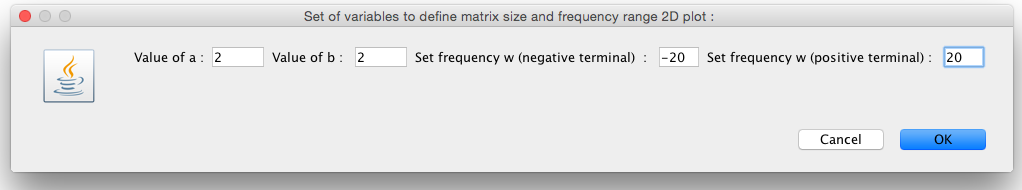
\includegraphics[width=0.8\textwidth]{figures/chap2/spinal1.png}
\caption{Main menu of the SpinAl software with parameters selection for stochastic indexes and frequency range.}
\label{figure:SpinAl1}
\end{figure}
For this specific example we set $a$ and $b$ as 2. Frequency range as $-20\leq\omega\leq 20$. Fixed magnetic field as 4 and fluctuating magnetic field along z-axis with a value of 3. transition rate value was randomly chosen as 0.01. We will describe in more details why this parameters were used and more details on the Hamiltonian derivation and Lioville matrix population at section\ref{blumeinitialmodel} 
\begin{figure}[h!]
\centering
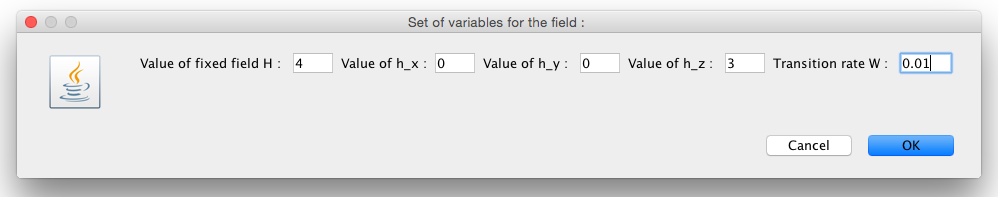
\includegraphics[width=0.8\textwidth]{figures/chap2/spinal2.png}
\caption{Proceeding menu of the SpinAl software with parameters selection for applied and fluctuating magnetic field as well as transition rate $W$.}
\label{figure:SpinAl2}
\end{figure}
\begin{figure}[h!]
\centering
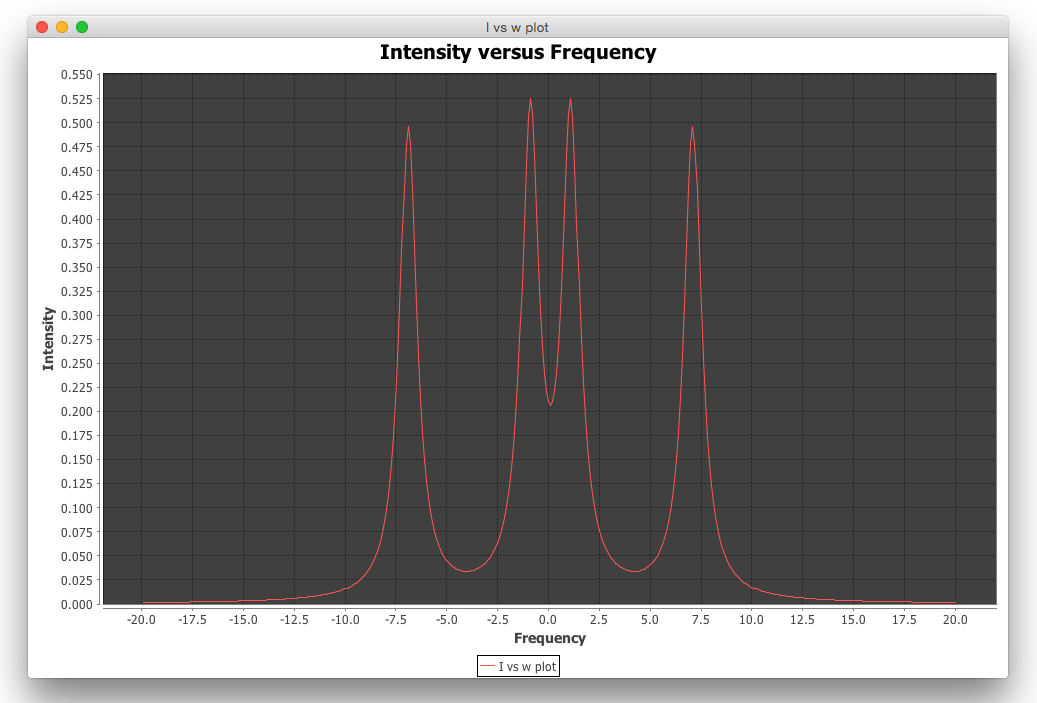
\includegraphics[width=0.8\textwidth]{figures/chap2/spinal3.png}
\caption{Produced graph of the Intensity versus Frequency after all model parameters have been entered.}
\label{figure:SpinAl3}
\end{figure}
Output of the computation will be Intensity versus frequency graph as on Fig.\ref{figure:SpinAl3}. \\
Currently SpinAl limited 2, 6 and 48 stochastic indexes as transition rate matrix under rotations is developed for this specific cases. We plan to generalize the software in future releases by adding possibility of creating custom $W$-matrix as well as rotation angles that could be uploaded as text files and parsed by SpinAl. Source code is available at authors public GitHub repository under open license\cite{nmrgit}.\\
The core algorithm of SpinAl to invert N-d arrays has been separated into framework available on separate GitHub repository\cite{ndgit}. It supports up to 10-D complex arrays inversion. Maximum size supported arrays size is limited precisely as: \ Array[100][100][10][10][10][10][10][10][10][10].\\
While working on SpinAl during mine PhD career our group was also exploring another possibilities to make computations cost-efficient. Thus we have successfully ported SpinAl to Python programming language where N-d array inversion was overcome by using native methods from scientific libraries. Python is a multi-paradigm high level cross-platform programming language that is well known for its relative simplicity of the syntax and fast expanding open source committing community. It is slower then Java~\cite{slower}. Core libraries like NumPy and SciPy \cite{scipy} for linear algebra make it relatively fast to perform system prototyping~\cite{SciPy1}~\cite{SciPy2}. Algebraic manipulations on N-Dimensional arrays are available in NumPy \cite{numpy} and two different algorithms on reshaping arrays in Fortran-like and C-like are available. Most of the well used libraries written for purpose of Magnetic Resonance computer simulations are given in Fortran code and using Python code wrapper it is possible to efficiently use the out of the box. We have also explored possibility of GPU~\cite{gpu} as well. The key results of this work will be mostly done in Python.\\*
We have also developed numerous useful tolls for proof-of-concept as well as transition rate matrix population in Matlab which are available upon request from Professor Keith Earle Lab. Matlab is a widely know in computational community multi-paradigm proprietary language developed by MathWorks and requires licence to use it. Matlab 8.2 R2013B was used to for the SpinAl algorithm implementation as well but had a lower performance to the equivalent in written Java. Using C-like N-dimensional array inversion available in latest releases I was not able to reproduce generalized results as in Java and Python in high magnetic field and lower transition rates regimes. Thus majority of the discussed results were obtained in Java and mostly in Python. Python source code is available at GitHub repository as well~\cite{eprgit}\\*
For computation purposes Asus ROG G75VX laptop was used with Intel 3rd generation Core i7 3630QM  processor, 16 GB DDR3 1600GHz memory and equipped with NVIDIA GTX 670 MX graphic processing unit(960 cores).\\* 
\subsection{Transition Rate Matrix}\label{trmsection}
In order to advance in description of the interacting environment well discussed in section \ref{kuboandersonsection} we need to determine suitable number of stochastic states $a$ and $b$ that form a two dimensional matrix $W$ known as transition rate matrix. We will start introduction from pure probabilistic approach with correlation to spin dynamics. We were discussing computational algorithm performance in a previous section but have not yet established the relation between 2,6 and 48 sotchastic indexes and their significance. Our goal in this research work was to determine lower bound of discrete states that are necessary to faithfully reproduce an ESR lineshape using concepts derived from information geometry\cite{Earle2009}.\\*
As an example of transition rate matrix construction we will start by introducing a two-state system that can uniformly and randomly transit between its states. As an example of such system one can imagine a chemical exchange where nucleus moves reversably from one environment to another at constant rate. In general this probabilistic approach on describing time evolution of of large discrete fluctuating systems is widely used in economics\cite{Weidlich1992}. Lets assume that for the nucleus transition to one state is defined by the rate $\omega_{1\rightarrow2}$ and jump back as $\omega_{2\rightarrow1}$ or simply $\omega_{12}$ and $\omega_{21}$. Corresponding probabilities are $P_{1}(t)$ and $P_{2}(t)$ that nucleus either in one or another state. We take the Markov assumption such that transition rate between states does not depend on the history of the process but rather on the state at specific time $t$ between enclosed time intervals $(t,t+dt)$. Further the probability of a nucleus being in state 1 between $(t,t+dt)$ can be described as following: 
\begin{equation}\label{eq:premaster}
P_{1}(t+dt)=P_{1}(t)[1-\omega_{12}dt]+P_{2}\omega_{21}dt+\mathcal{O}(dt^2)
\end{equation} 
First term arises from assumption that nucleus did not transition to the second state and second term represents transition back to the state 1 in a given time interval. The last term $\mathcal{O}(dt^2)$ came from assumption that particle could follow a chain from $1\rightarrow 2 \rightarrow 1$. Taking a limit $dt\rightarrow 0$ the result appear to be a simple set of differential equations: 
\begin{equation}\label{eq:masterlol}
\frac{dP_{1}}{dt}=-\omega_{12}P_{1}(t)+\omega_{21}P_{2}(t)
\end{equation}
Or generalized we can writte for arbitary states as: 
\begin{equation}\label{eq:master}
\frac{dP_{i}}{dt}=-\sum_{j\neq i}\omega_{i\rightarrow j}P_{i}+\sum_{j\neq i}\omega_{j\rightarrow i}P_{j}
\end{equation}
Eq.\ref{eq:master} known as Master Equation. In vector form:   
\begin{equation}\label{eq:matrix}
\frac{d\vec{p}}{dt}=-\vec{W}\vec{p}
\end{equation} 
Where $\vec{p}$ is a column vector with probabilities $p_i$ and $\vec{W}$ is a square transition rate matrix.
 Solution of master equation requires eigencalues and vectors calculation of martix $W$ which can be a difficult task for large stochastic systems. Also not that digonal elemts of $W$ defined as:  
\begin{equation}\label{eq:markov3}
-W_{i,i}\equiv\sum_{j,j\neq i}W_{i,j}
\end{equation} 
Accordingly we can construct two-state system transition matrix as following:   
\begin{equation}\label{eq:55}
W = \begin{bmatrix}
       -w_{11} & w_{12}  \\[0.3em]
        w_{21} & -w_{22}  
     \end{bmatrix}
\end{equation}
Diagonal elements are defined via Eq.\ref{eq:markov3} and it means that probability leaving the state is equal to the probability of reaching it. In more complicated example whn relaxation processes couples more states due to the complicated spin motion pattern consider 6 possible states(events). Graph of allowed transitions is given on Fig.\ref{figure:wdiagramm}. One can imagine an octahedron in three dimensional representation labelling edges with indexes from 1 to 6 and defining adjacency matrix of relative coupling,    
\begin{figure}[h!]
\begin{center}
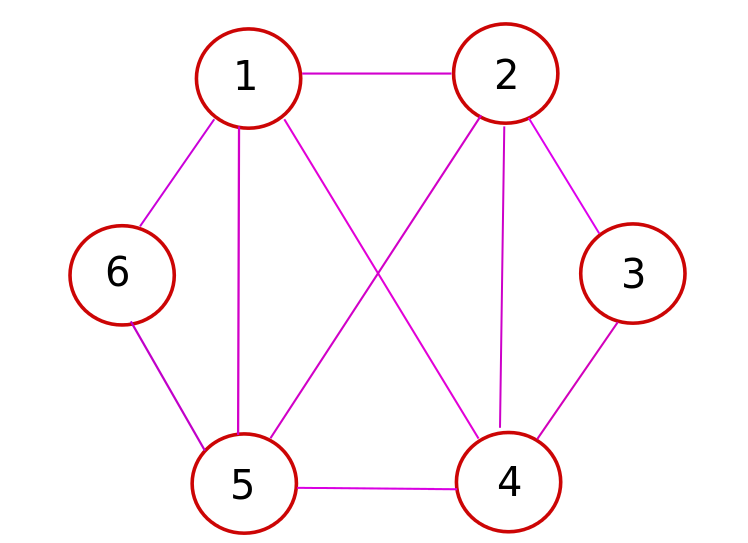
\includegraphics[width=0.7\textwidth]{figures/chap2/wdiagramm.png}
\caption{transition probabilities graph between 6 possible events}
\label{figure:wdiagramm}
\end{center}
\end{figure}
\begin{equation}\label{eq:Wmat1}
W = \begin{bmatrix}
       w_{11} & w_{12} & 0 & w_{14} & 0 & w_{16}  \\[0.3em]
       w_{21} & w_{22} & w_{23} & 0 & w_{25} & 0  \\[0.3em]
       0 & w_{32} & w_{33} & w_{34} & w_{35} & 0  \\[0.3em]
       w_{41} & 0 & w_{43} & w_{44} & w_{45} & 0 \\[0.3em]
       0 & w_{52} & 0 & w_{54} & w_{55} & w_{56} \\[0.3em]
       w_{61} & 0 & w_{63} & 0 & w_{65} & w_{66} 
     \end{bmatrix}
\end{equation}
Diagonal elements are defined as well as for 2 events case by Eq.\ref{eq:markov3}. Another interest is to define rate of tumbling between probability of transitions and assume that an a priori probability between different states transitions might not equal to each other. More evidentially assume transformation of principal axis frame of $g$ or $A$ tensors that are parametrized by euler angles and define  fast transition as $\vec{R}(0,0,0)\xrightarrow {1\rightarrow 6}\vec{R}(0,0,\pi/2)$. Similarly moderate $\vec{R}(0,0,0)\xrightarrow {1\rightarrow 2}\vec{R}(0,\pi/2,0)$  and slow $\vec{R}(0,0,0)\xrightarrow {1\rightarrow 4}\vec{R}(0,0,\pi/2)$. The results for the constructed matrix is given below,   
\begin{equation}\label{eq:Wmat2}
W = \begin{bmatrix}
       0 & m & 0 & s & 0 & f  \\[0.3em]
       m & 0 & s & 0 & f & 0  \\[0.3em]
       0 & s & 0 & f & m & 0  \\[0.3em]
       s & 0 & f & 0 & m & 0 \\[0.3em]
       0 & f & 0 & m & 0 & s \\[0.3em]
       f & 0 & m & 0 & s & 0 
     \end{bmatrix}
\end{equation}
Where $s,m$ and $f$ define three probability transition rates: slow, moderate and fast respectively. It appears that for special cases it might slightly modify the line shape. Yet another even more complicated case is given as 48 total stochastic states defined by quaternion representation by rotation by $\pi/2$ on $S(3)$ assuming nearest neighbours distance as $pi/4$ and Euler angles have been reconstructed. The output of the adjacent matrix is appeared to be sparse
\begin{figure}[h!]
\begin{center}
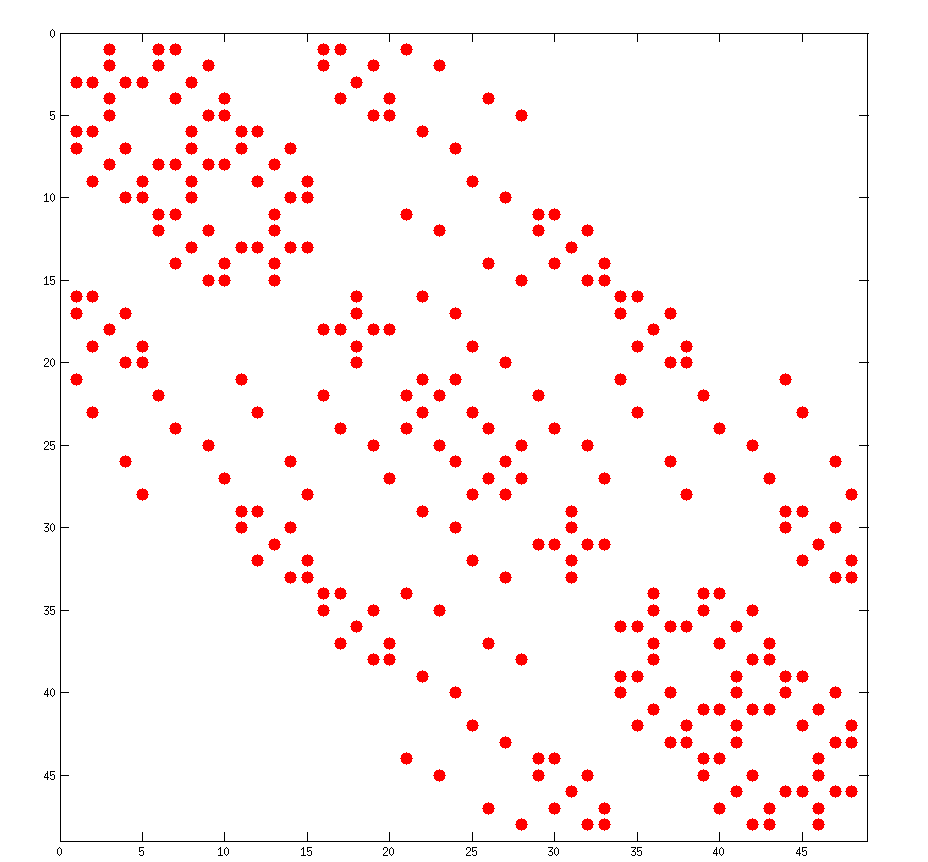
\includegraphics[scale=0.5]{figures/chap2/sparce.png}
\caption{Illustration of allowed transitions between 48 states defined by quaternion representation of  rotation os $S(3)$. Allowed transitions are in red. }
\label{figure:blumediag}
\end{center}
\end{figure}  
\clearpage
\subsection{Chemical Shift}\label{blumeinitialmodel}
Validation step for validation AI algorithm is to reproduce original absorption spectra of NMR linehshape for isolated spin-1/2 nucleus in a fixed magnetic field and fluctuating fields along $x,y$ and $z$ orientations. For specific model $I_0=I_1=1/2$. Number of stochastic states corresponds to two and can be described as chemical exchange process. As simple example of chemical exchange consider two $N$-methyl groups in $N,N'$ - dimethylformamide can exchange their relative bond and reactant chemically and physically remains indistinguishable from the product. Methyl groups are coloured in red and black to make process visible.       
\begin{figure}[h!]
\centering
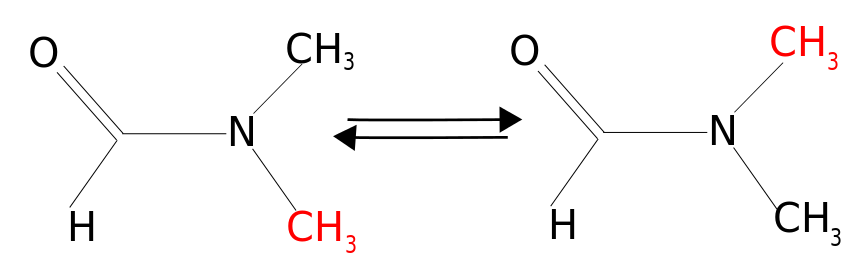
\includegraphics[width=0.7\textwidth]{figures/chap2/methil.png}
\caption{$N,N'$ -
dimethylformamide chemical exchange of methyl groups in active moiety.}
\label{figure:methyl}
\end{figure}
Magnetic environment of $N$-methyl groups will be different after the chemical exchange which leads to the fact that they will have different resonance frequencies before and after the reaction and molecular motion can be treated by Blume stochastic model. Example of the NMR spectra dependence on temperature is given on Fig.\ref{figure:datamet} 
\begin{figure}[h!]
\begin{center}
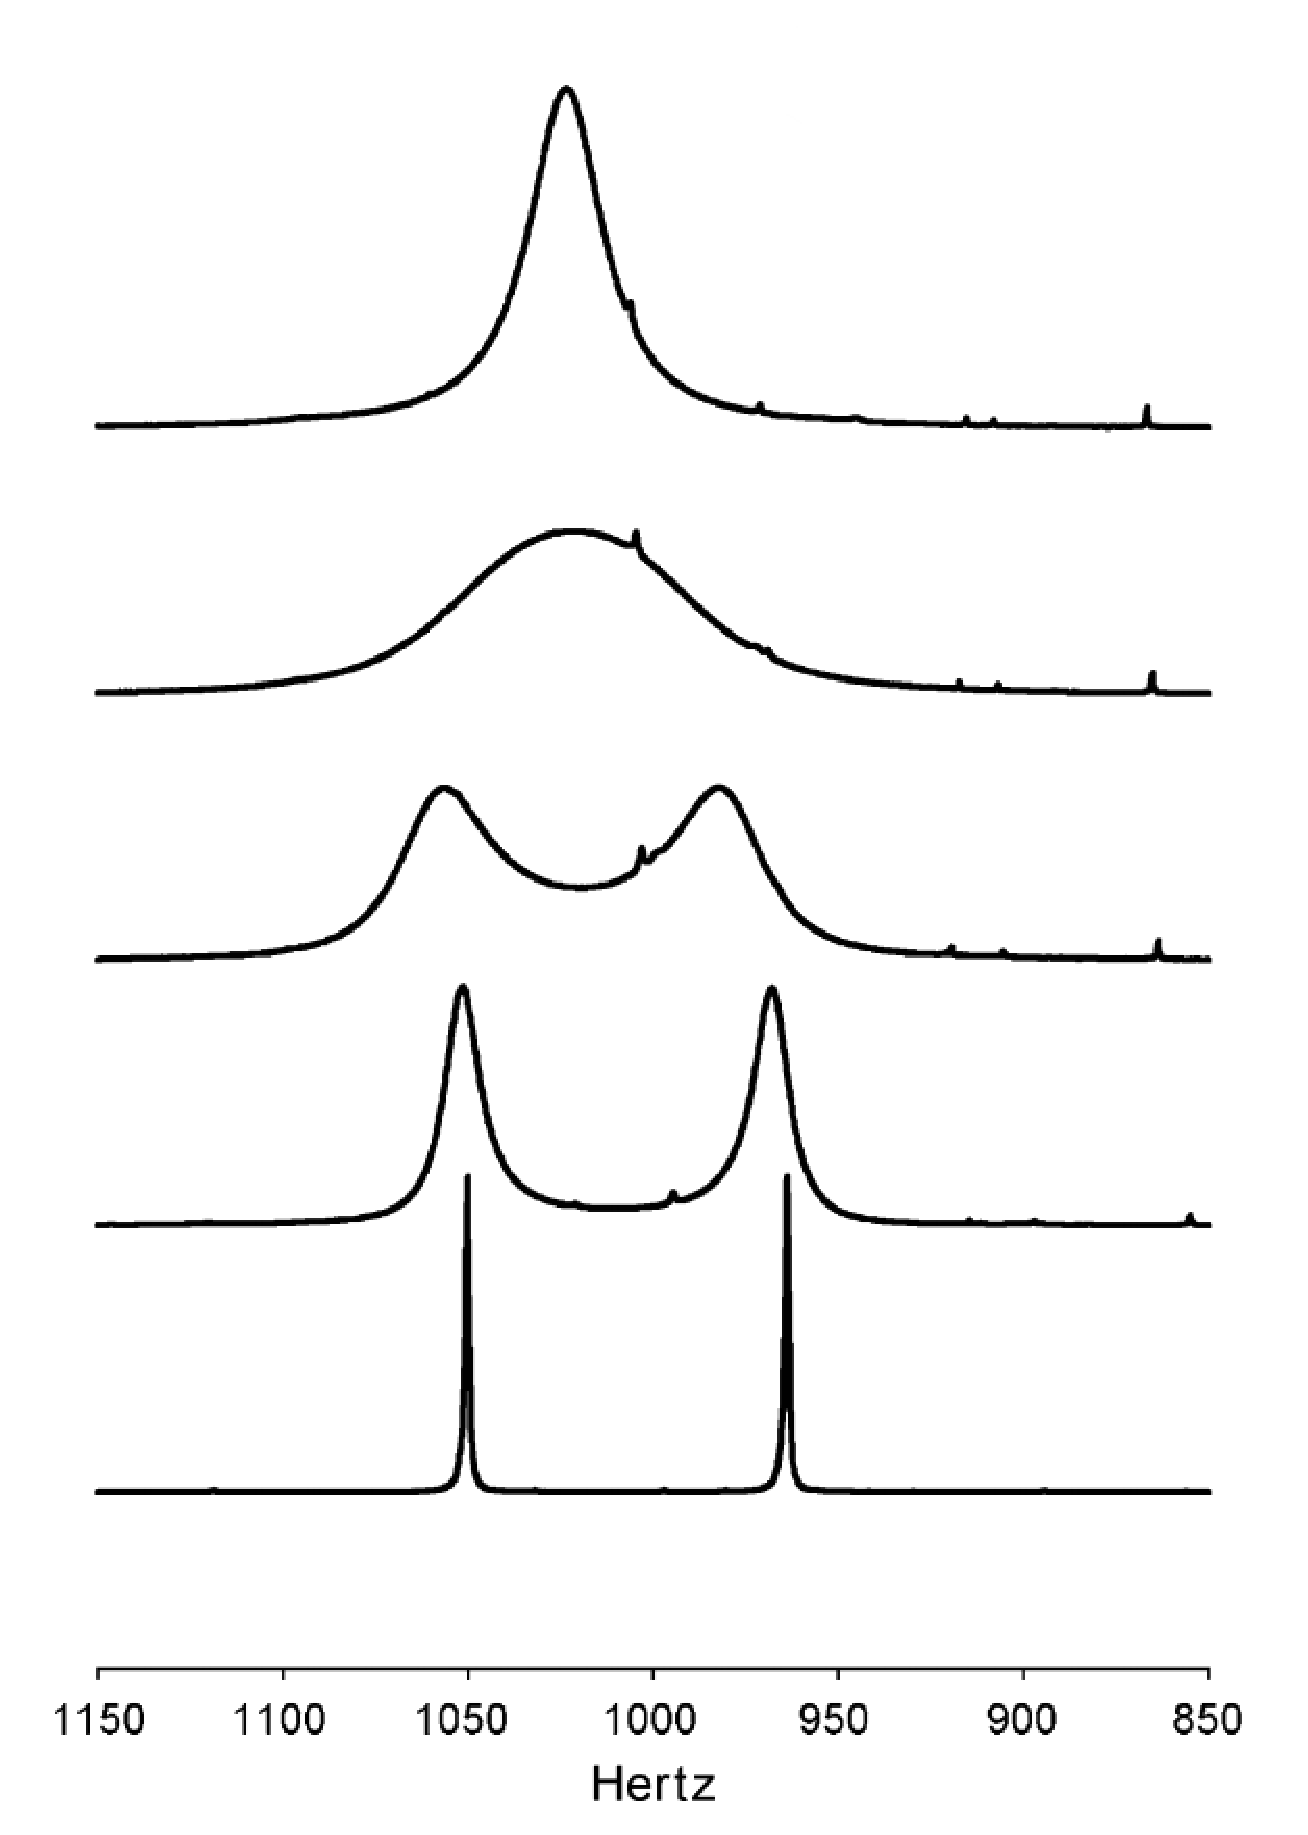
\includegraphics[scale=0.5]{figures/chap2/methyldat.eps}
\caption{"Proton NMR spectra at 300 MHz of the $N$-methyl signals in a
derivative of azapropazone as a function of temperature. The lowest spectrum is at 223 K, and then
at 243, 253, 263, and 273 K"~\cite{Bain200363}}
\label{figure:datamet}
\end{center}
\end{figure}  
Treatment of simple molecular motions and chemical exchange well described in Gamilel ~\cite{gamilel} where they start from determination of absorption spectra by analogy of finding correlation function of classical harmonic oscillator similar to Kubo, Anderson and Blume treatment. Stochastic matrix $W$ introduced in Eq. \ref{eq:34},\ref{eq:35} and \ref{eq:37}that defines transition probability per unit time between stochastic states $a$ and $b$ has the following form:  
For this specific example $p_a=p_b=1/2$. Derivation of proper $W$ matrix and assigning a priori probabilities is a key to correct computation of absorption spectra for complex dynamic environment.Assuming that a priori probabilitieas are equal transition rate is uniform for between the transitions so that $w_{a,b}=w_{b,a}=T$ where $T$ is a transition rate \\*
Time dependent Hamiltonian in Blume\cite{blume} represents nuclear Zeeman interaction and can be constructed as following: 
\begin{equation}\label{eq:58}
\mathcal{H}(t)=\sum_jV_jf_j(t)=B_0I_z+\vec{h}\cdot\hat{I}f(t)
\end{equation}  
Fixed magnetic field $B_0$ by NMR and EPR convention in this case is set along $z$ axis and fluctuating local field $h(x,y,z)$ can point in any arbitrary direction. Stochastic function $f(t)$ can take two values 1 or -1. In feasable form Eq. \ref{eq:58} can be written as: 
\begin{equation}\label{eq:blumeham}
\mathcal{H}(t)=B_0I_z+f(t)\big[\frac{1}{2}(h_+I_-+h_-I_+)+h_zI_z\big]
\end{equation}     
Where $I_{\pm}$ are rising and lowering nuclear spin operators and $h_{\pm}=h_x\pm h_y$ and $h_z$ defines fluctuating field in assosiated with spin operators in $x,y,z$ planes. \\*
Dimension of Liouville matrix is $8\times 8$ and its precise and accurate construction from Eq. \ref{eq:35} is presented in Eq.\ref{eq:60}. In the case when local fluctuating fields aligned with the applied field $h_+=h_-=0$ matrix Eq.\ref{eq:60} reduces to banded or sparse matrix with two non-zero diagonals Eq.\ref{eq:61}. Thus $8\times 8$ matrix reduce to four $2\times 2$ and from computational prospective it is possible to take to account only the two middle matrices and invert them separately which is less time consuming. This is not always the case and in EPR and off-diagonal elements can carry important structural information. \\*
Following procedure from Blume \cite{blume} fixed field was set to $B_0=3$ and fluctuating field $h=h_x=h_y=h_z=4$. Results are presented on Fig.\ref{figure:blumediag}. For all (a), (b) and (c) for fast modulation regime line shape is represented by sharp Lorentizan peak centred around Zeeman frequency. At shorter transition rates thus slow relaxation regime case (a) and (b) represent absorption spectra with fluctuating local fields along $x$ and $y$ axis. The peak roughly occurs at $\omega\approx(B_0^2+h^2)^{1/2}$. Additional Broad side peak at  Fig.\ref{figure:blumediag}(a) can be explained as image of electric non-static Gaussian electron field strength distribution. For the case at Fig.\ref{figure:blumediag}(c) fluctuating field along $z$ axis and two lines correspond to each of the two state frequencies defined as $\omega\approx B_0\pm h$. Fig.\ref{figure:blumediag}(c) corresponds to classical example of temperature dependence of NMR and EPR spectrum due to chemical exchange. In all three cases with the increasing of transition rates lines are broadening at some moderate rate and then collapse into one narrowed line as change of stochastic transitions averages out. \\*
Simulated figures at Fig.\ref{figure:blumediag}(c) completely agrees with originally proposed by Blume \cite{blume} and were obtained by manually typing Liouville matrix and performing inversion and summation to obtain absorption spectra and by AI generalized algorithm. Both computational cases converged to one solution which was an indicator of AI validity and robustness.           
           
\clearpage
\begin{landscape}
\begin{equation}\label{eq:60}
\mathcal{L} = \begin{bmatrix}
       p-w_{aa} & -w_{ab} & \frac{1}{2}h_+ & 0 & -\frac{1}{2}h_- & 0 & 0 & 0  \\[0.3em]
       -w_{ba} & p-w_{bb} & 0 & -\frac{1}{2}h_+ & 0 & \frac{1}{2}h_- & 0 & 0  \\[0.3em]
       \frac{1}{2}h_- & 0 & p-w_{aa}-i(B_0+h_z) & -w_{ab} & 0 & 0 & -\frac{1}{2}h_- & 0  \\[0.3em]
       0 & -\frac{1}{2}h_- & -w_{ba} & p-w_{bb}-i(B_0-h_z) & 0 & 0 & 0 & \frac{1}{2}h_-  \\[0.3em]
       -\frac{1}{2}h_+ & 0 & 0 & 0 & p-w_{aa}-i(B_0+h_z) & -w_{ab} & \frac{1}{2}h_+ & 0  \\[0.3em]
       0 & \frac{1}{2}h_+ & 0 & 0 & -w_{ba} & p-w_{bb}+i(B_0-h_z) & 0 & -\frac{1}{2}h_+  \\[0.3em]
       0 & 0 & -\frac{1}{2}h_+ & 0 & \frac{1}{2}h_- & 0 & p-w_{aa} & -w_{ab}  \\[0.3em]
       0 & 0 & 0 & \frac{1}{2}h_+ & 0 & -\frac{1}{2}h_- & -w_{ba} & p-w_{bb} 
     \end{bmatrix}
\end{equation}
\end{landscape} 

\begin{landscape}
\begin{equation}\label{eq:61}
\mathcal{L} = \begin{bmatrix}
       p-w_{aa} & -w_{ab} & 0 & 0 & 0 & 0 & 0 & 0  \\[0.3em]
       -w_{ba} & p-w_{bb} & 0 & 0 & 0 & 0 & 0 & 0  \\[0.3em]
       0 & 0 & p-w_{aa}-i(B_0+h_z) & -w_{ab} & 0 & 0 & 0 & 0  \\[0.3em]
       0 & 0 & -w_{ba} & p-w_{bb}-i(B_0-h_z) & 0 & 0 & 0 & 0  \\[0.3em]
       0 & 0 & 0 & 0 & p-w_{aa}-i(B_0+h_z) & -w_{ab} & 0 & 0  \\[0.3em]
       0 & 0 & 0 & 0 & -w_{ba} & p-w_{bb}+i(B_0-h_z) & 0 & 0  \\[0.3em]
       0 & 0 & 0 & 0 & 0 & 0 & p-w_{aa} & -w_{ab}  \\[0.3em]
       0 & 0 & 0 & 0 & 0 & 0 & -w_{ba} & p-w_{bb} 
     \end{bmatrix}
\end{equation}
\end{landscape} 

\begin{figure}[h!]
\centering
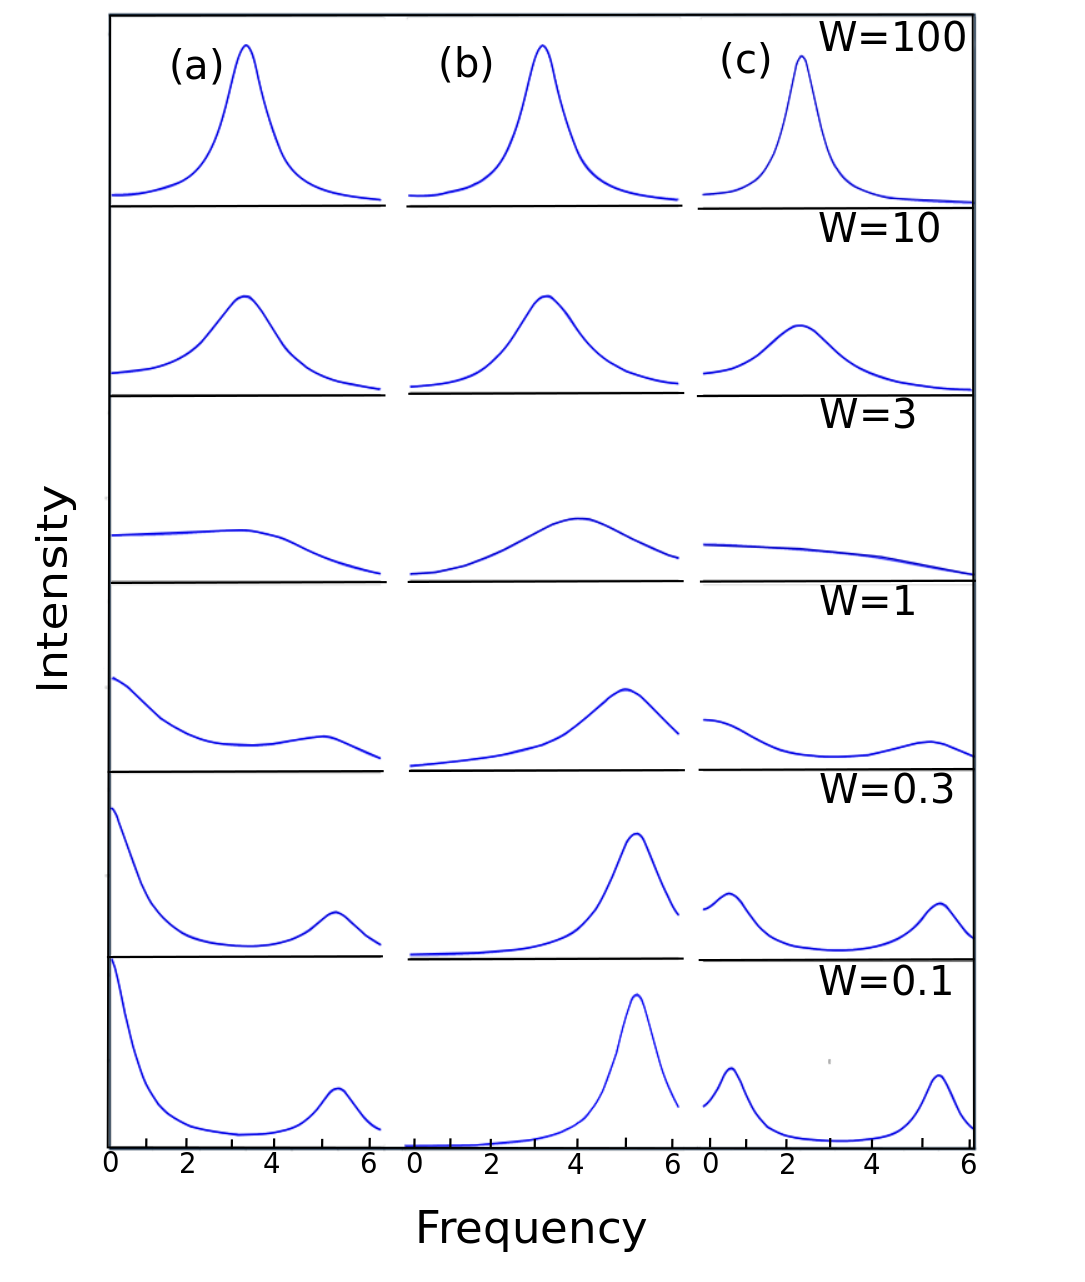
\includegraphics[width=0.7\textwidth]{figures/chap2/blumediag.png}
\caption{Evolution of NMR line shapes with increase of transition rates $W$ for $I=1/2$ nucleus in a fixed magnetic field along $z$ axis and fluctuating local magnetic fields $h$ along (a) $x$ axis, (b) $y$ axis and (c) $z$ axis. Simulated using AI alagorithm}
\label{figure:blumediag}
\end{figure}
\clearpage
\subsection{Anisotropic Zeeman}\label{zeemansection}
To examine if the model is valid for axial asymmetric contributing terms of Hamiltonian first proper construction inculding orientation dependence should be made. Effective anisotropic Hamiltonian for isolated unpaired electron in tensor contraction form using Eq.\ref{eq:58} and Eq.\ref{eq:60} with $g$-tensor components transformed into the laboratory frame\cite{NMRtomograph}\cite{Nordio} using Eq.\ref{eq:47}:
\begin{subequations}\label{eq:48}
\begin{align}
A^{[2],L}_{\pm2,(g)} & =-\frac{1}{2}S_{\pm}B_{\pm}\\
A^{[2],L}_{\pm1,(g)} & =\pm\frac{1}{2}(S_{\pm}B_{z}+S_zB_{\pm})\\
A^{[2],L}_{0,(g)} & =-\sqrt{\frac{2}{3}}\big(S_{z}B_{z}-\frac{1}{4}(S_+B_-+S_-B_+)\big)\\
A^{[0],L}_{0,(g)} & =\frac{1}{\sqrt{3}}\big(S_{z}B_{z}+\frac{1}{2}(S_+B_-+S_-B_+)\big)
\end{align}
\end{subequations}
Where $B_{\pm}=B_x\pm iH_y$. Choosing applied magnetic filed being oriented along $z$ axis in the laboratory frame  Eq.\ref{47}a and Eq.\ref{eq:47}b are vanishing: 
\begin{subequations}\label{eq:49}
\begin{align}
A^{[2],L}_{\pm2,(g)} & =0\\
A^{[2],L}_{\pm1,(g)} & =0\\
A^{[2],L}_{0,(g)} & =-\sqrt{\frac{2}{3}}S_{z}B_{z}\\
A^{[0],L}_{0,(g)} & = \frac{1}{\sqrt{3}}(S_{z}B_{z}
\end{align}
\end{subequations}
The $g$-tensor decompose into rank-zero tensor $g^{(0,0)}$ and five components of second-rank tensor $g^{(2,m)}\rightarrow(g^{(2,\pm2)}, g^{(2,\pm1)},g^{(2,0)})$. Writing in principal axis frame IST components are: 
\begin{subequations}\label{eq:50}
\begin{align}
F^{[2],P}_{\pm2,(g)} & =-\frac{1}{2}\beta_e(g_{xx}-g_{yy})\\
F^{[2],P}_{\pm1,(g)} & =0\\
F^{[2],P}_{0,(g)} & =-\sqrt{\frac{2}{3}}\beta_e\big(g_{zz}-\frac{1}{2}(g_{xx}-g_{yy})\big)\\
F^{[0],P}_{0,(g)} & = \frac{1}{\sqrt{3}}\beta_e(g_{xx}+g_{yy}+g_{zz})
\end{align}
\end{subequations}
From the definition:
\begin{equation}
F^{[2],L}_{m,g}=\sum_{m'}(-1)^m(\mathcal{D}^{[2]}_{m,m'}(\alpha,\beta,\gamma))^*F^{[2],P}_{m',g}
\end{equation}
And using Wigner matrix elements from Tab.\ref{tab:wigner} in simple form:  
\begin{multline}\label{eq:tensorzeem}
F^{[2],L}_{m,g}=(-1)^m\Big(\big(\mathcal{D}^{[2]}_{m,2}(\alpha,\beta,\gamma)+\mathcal{D}^{[2]}_{m,-2}(\alpha,\beta,\gamma))F^{[2],P}_{2,g}+\mathcal{D}^{[2]}_{m,0}(\alpha,\beta,\gamma)F^{[2],P}_{0,g}\Big)= \\ =(-1)^m\Big((e^{im\alpha}d_{-m,2}^2(\beta)e^{-i2\gamma}+e^{im\alpha}d_{-m,2}^2(\beta)e^{i2\gamma}) F^{[2],P}_{2,g}+e^{im\alpha}d_{-m,0}^2(\beta)F^{[2],P}_{0,g}\Big)
\end{multline}
And finally in terms of matrix elements for $m=-2...2$
\begin{subequations}\label{eq:dmatel}
\begin{align}
F^{[2],L}_{-2,g}& = e^{-i2\alpha}\Big[(\frac{1+\cos^2\beta}{2}\cos2\gamma-i\cos\beta\sin2\gamma) F^{[2],P}_{2,g}+\sqrt\frac{3}{8}\sin^2\beta F^{[2],P}_{0,g} \Big]\\
F^{[2],L}_{-1,g}& = -e^{-i\alpha}\Big[(\cos\beta\cos\beta\cos2\gamma-i\sin\beta\sin2\gamma) F^{[2],P}_{2,g}+\sqrt\frac{3}{2}\sin\beta\cos\beta F^{[2],P}_{0,g} \Big]\\
F^{[2],L}_{0,g}& = \sqrt\frac{3}{2}\sin^2\beta\cos2\gamma F^{[2],P}_{2,g}+\frac{1}{2}(3\cos^2\beta-1)F^{[2],P}_{0,g} \\
F^{[2],L}_{1,g}& = e^{i\alpha}\Big[(\cos\beta\cos\beta\cos2\gamma+i\sin\beta\sin2\gamma) F^{[2],P}_{2,g}+\sqrt\frac{3}{2}\sin\beta\cos\beta F^{[2],P}_{0,g} \Big]=(F^{[2],L}_{2,g})^*\\
F^{[2],L}_{2,g}& = e^{i2\alpha}\Big[(\frac{1+\cos^2\beta}{2}\cos2\gamma+i\cos\beta\sin2\gamma) F^{[2],P}_{2,g}+\sqrt\frac{3}{8}\sin^2\beta F^{[2],P}_{0,g} \Big]=(F^{[2],L}_{2,g})^*
\end{align}
\end{subequations}
To summarize the Hamiltonian in the comlicated case for assymetric $g$-tensor including both "secular" and "non-secular" terms: 
\begin{equation}
\mathcal{H}_{eff}=A_0^{[0]}F_0^{[0]}+A_0^{[2]} F_0^{[2]}+A_{+2}^{[2]} F_{+2}^{[2]}+A_{-2}^{[2]} F_{-2}^{[2]}
\end{equation}
For non-saturated lines it is enough to include only "secular" part which is the interaction term proportional to $S_z$ operator bounding states to themselves. It is true if correlation time is short compared to inverse of the Larmor frequency. 
\begin{equation}
\mathcal{H}_{eff}=(\frac{1}{\sqrt{3}}S_zB_z)F_0^{[0]}+(-\sqrt\frac{2}{3}S_zB_z)F_0^{[2]}
\end{equation}
Simulated spectra for anisotropic $g$-tensor contribution with rhombic axial symmetry is presented on figure ~\ref{figure:gten1}. Spectra is extremely sensitive to the adjusting parameters of the model as well as transition rates. For example effect of rhombic symmetry is observable for the rates lower then $0.05$othervise the one Lorentzian peak is observed. Resolution should be set no lower then 0.01 othervise the same Lorentzian line shape is presented. 
\begin{figure}[h!]
\centering
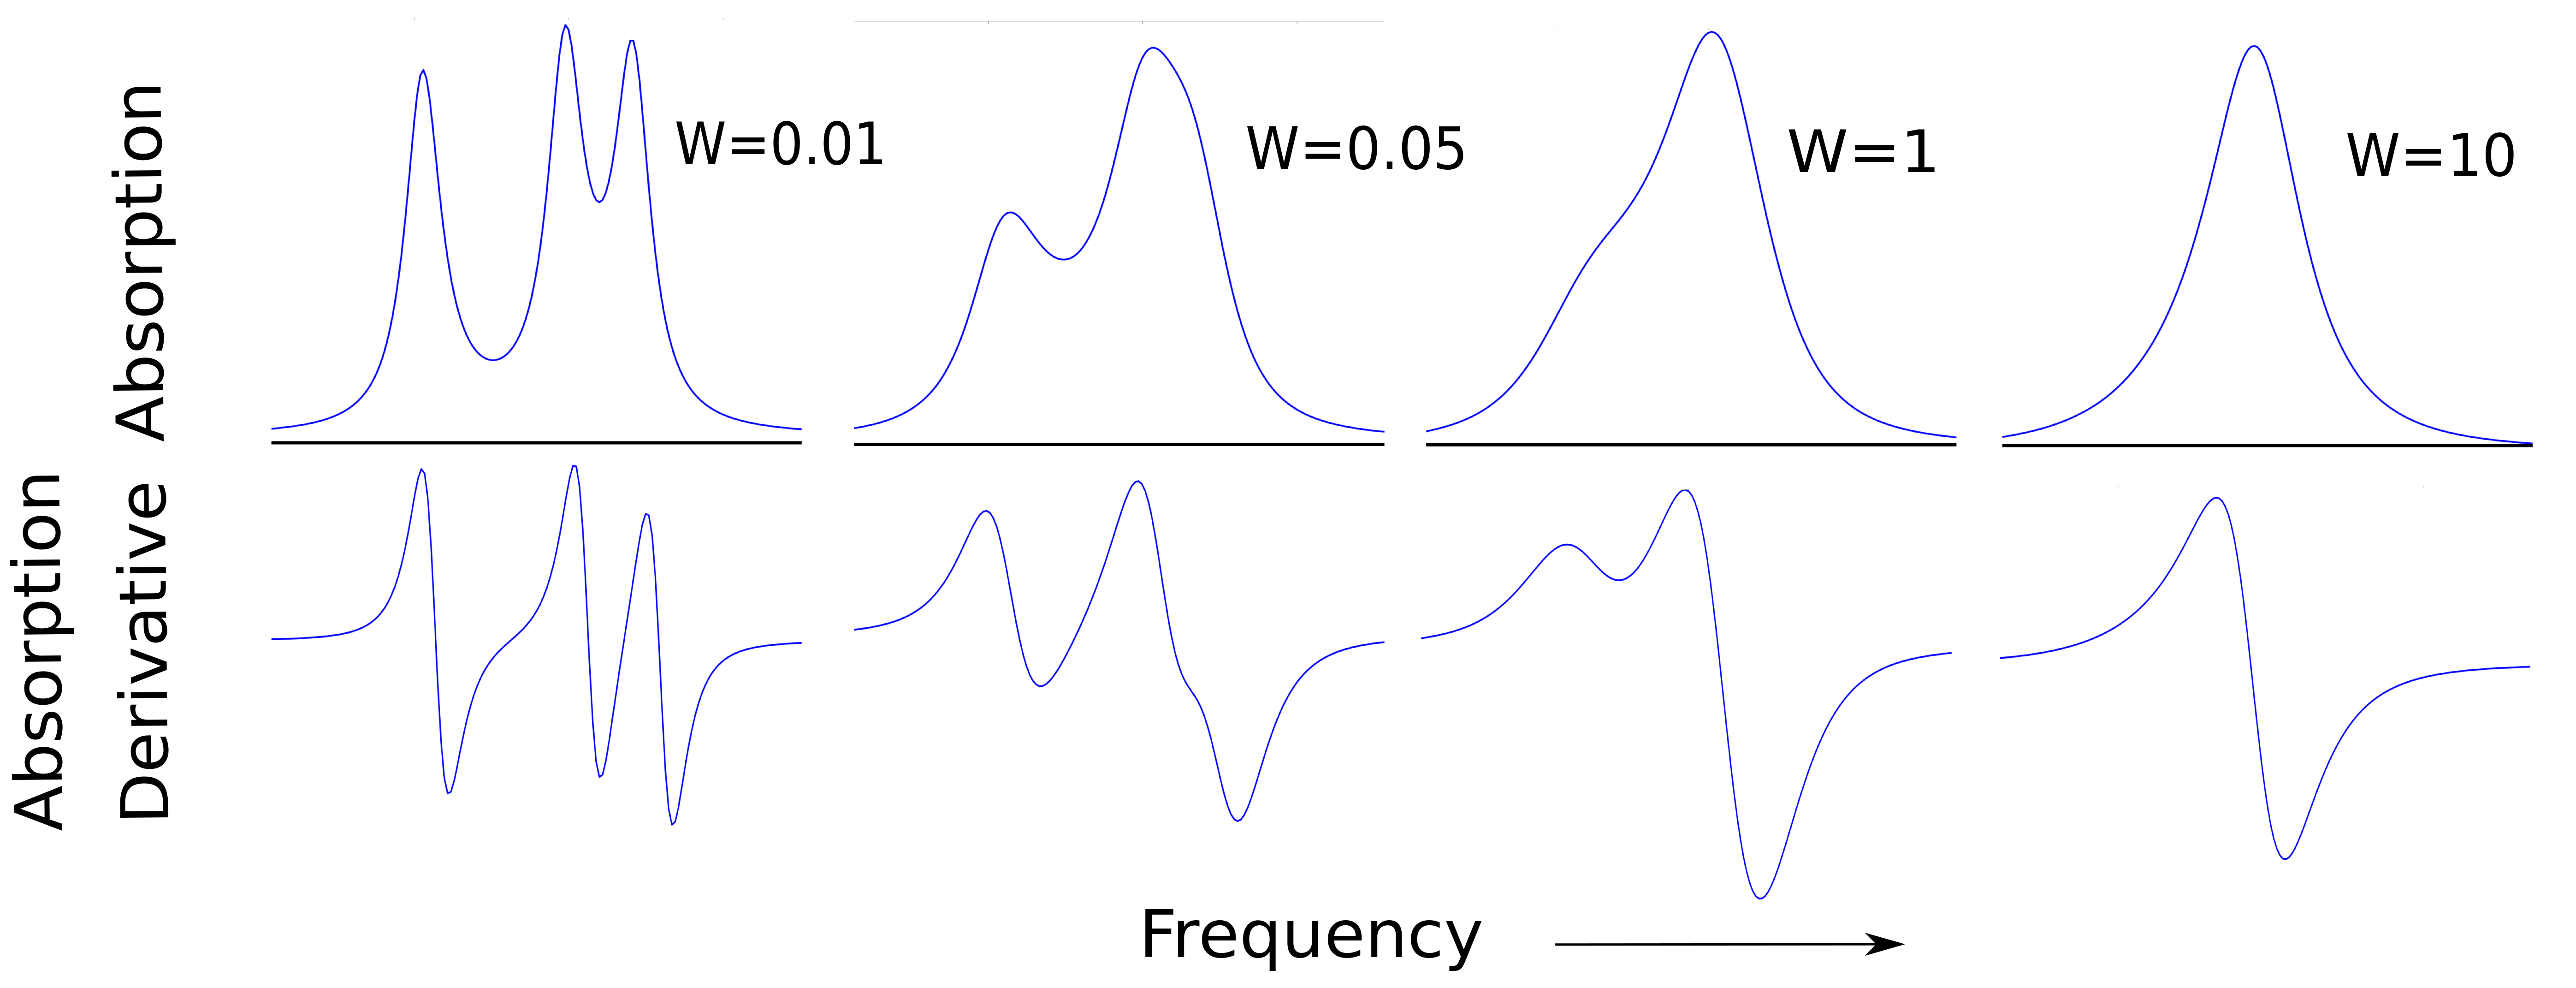
\includegraphics[height=8cm,width=1\textwidth]{figures/chap2/gtenanisat1.png}
\caption{Evolution of NMR line shapes with increase of transition rates $W$ for $I=1/2$ nucleus in a fixed magnetic field along $z$ axis and fluctuating local magnetic fields $h$ along (a) $x$ axis, (b) $y$ axis and (c) $z$ axis. Simulated using AI alagorithm}
\label{figure:gten1}
\end{figure}
There are no significant differences between 6 and 48 stochastic brining computational relief to us. 
\begin{figure}[h!]
\centering
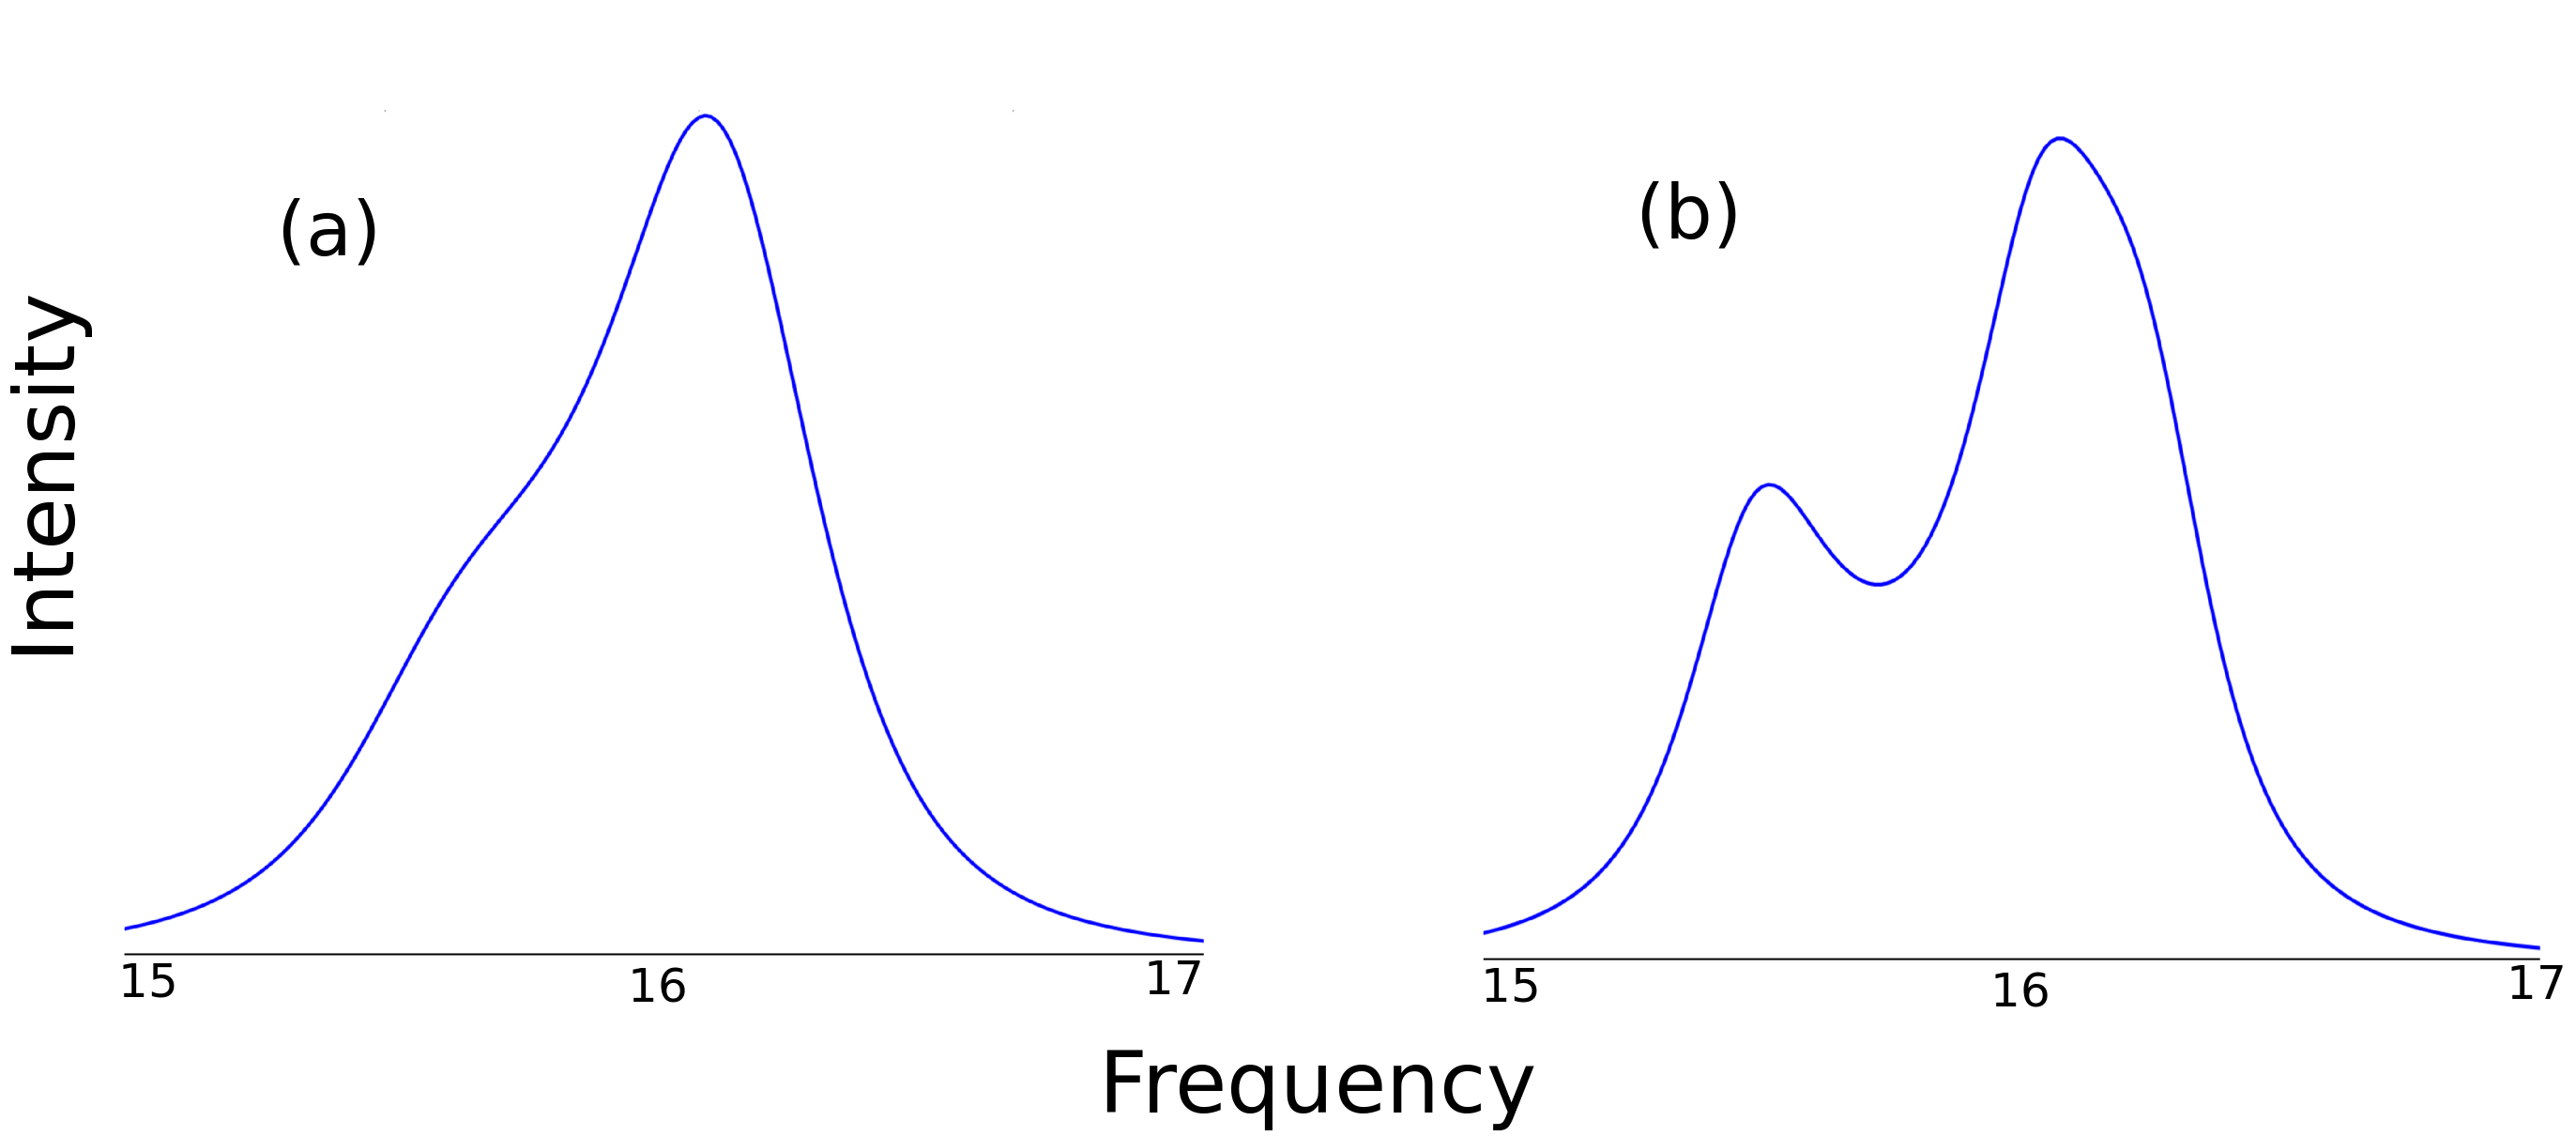
\includegraphics[height=8cm,width=1\textwidth]{figures/chap2/gtenanisat2.png}
\caption{Evolution of NMR line shapes with increase of transition rates $W$ for $I=1/2$ nucleus in a fixed magnetic field along $z$ axis and fluctuating local magnetic fields $h$ along (a) $x$ axis, (b) $y$ axis and (c) $z$ axis. Simulated using AI alagorithm}
Interestingly that using unequal a priori probability between states transition and using transition rates matrix designed in Eq.\ref{eq:Wmat2} setting $s=0.1,m=1$ and $f=100$ line shape tend to represent the case of axial symmetry or that $g_{xx}=g_{yy}<g_{zz}$ 
\label{figure:gterates}
\end{figure}
\clearpage
\subsection{Coupled Spins 1/2}\label{05coupledspinsection}
The more complicated and fascinating interest for our group occurs when unpaired electron spin is interacting with nuclei. Thus a hyperfine interaction should be added. But first lets modify Eq.\ref{eq:37} adding additional sets of bra and kets for the unpaired electron quantum states $\langle m_{0s},m_{1s},S_0,S_1|$ and $|S_0,S_1,m_{0s}',m_{1s}'\rangle$ on both sides.  
\begin{multline}\label{eq:newbras}
P(\omega)=
\frac{2}{\Gamma(2I_0+1)}\mathcal{H}^{(-)}\delta_{m_{1I}m_{0I}}\delta_{m_{1S}m_{0S}}\mathcal{H}^{(+)}\delta_{m_{1I}'m_{0I}'}\delta_{m_{1S}'m_{0S}'} \\ \times[s\delta_{ab}\delta_{m_{1I}m_{1I}'}\delta_{m_{0I}m_{0I}'}\delta_{m_{1S}m_{1S}'}\delta_{m_{0S}m_{0S}'}-(a|W|b)\delta_{m_{0I}m_{0I}'}\delta_{m_{1I}m_{1I}'}\delta_{m_{0S}m_{0S}'}\delta_{m_{1S}m_{1S}'} \\ -i(a|F|a)\delta_{ab}[\langle I_0S_0m_{0I}m_{0S}|V_j|I_0S_0m_{0I}'m_{0S}'\rangle \delta_{m_{0I}m_{0I}'}\delta_{m_{0S}m_{0S}'}\\-\langle I_1S_1m_{1I}m_{1S}|V_j|I_1S_1m_{1I}'m_{1S}\rangle\delta_{m_{1I}m_{1I}'}\delta_{m_{1S}m_{1S}'}]^{-1}
\end{multline} 
Starting vectors $\mathcal{H}^{(+)}$ and $\mathcal{H}^{(-)}$ that define proper electronic magnetization components for the line shape are modified accordingly to \cite{bmr}: 
\begin{equation}
\langle \mathcal{H}^{(+)} \rangle=\langle S_x\otimes I_1 \rangle
\end{equation}
Where $I_1$ is a unit operator in nuclear spin space. $\langle S_x\rangle$ can be easily found in terms of rising and lowering operators and corresponding matrix constructed. \\*
Similarly to the ISTO transformation of the Zeeman part of Hamiltonian it is possible to write all components of the transformed hyperfine interaction term. Starting with spin operators in laboratory frame:   
\begin{subequations}\label{eq:hyperA}
\begin{align}
A^{[2],L}_{\pm2,(hf)} & =-\frac{1}{2}S_{\pm}I_{\pm}\\
A^{[2],L}_{\pm1,(hf)} & =\pm\frac{1}{2}(S_{\pm}I_{z}+S_zI_{\pm})\\
A^{[2],L}_{0,(hf)} & =-\sqrt{\frac{2}{3}}\big(S_{z}I_{z}-\frac{1}{4}(S_+I_-+S_-I_+)\big)\\
A^{[0],L}_{0,(hf)} & =\frac{1}{\sqrt{3}}\big(S_{z}I_{z}+\frac{1}{2}(S_+I_-+S_-I_+)\big)
\end{align}
\end{subequations}
Correspondingly principal components of the $A$-tensor: 
\begin{subequations}\label{eq:HyperAA}
\begin{align}
F^{[2],P}_{\pm2,(hf)} & =-\frac{1}{2}\beta_e(A_{xx}-A_{yy})\\
F^{[2],P}_{\pm1,(hf)} & =0\\
F^{[2],P}_{0,(hf)} & =-\sqrt{\frac{2}{3}}\beta_e\big(A_{zz}-\frac{1}{2}(A_{xx}+A_{yy})\big)\\
F^{[0],P}_{0,(hf)} & = \frac{1}{\sqrt{3}}\beta_e(A_{xx}+A_{yy}+A_{zz})
\end{align}
\end{subequations}
Transformation between laboratory and principal axis system for the hyperfine interaction can be done in similar fashion as for the $g$ tensor. Working in the linear response regime only commuting terms with the Zeeman Hamiltonian are of interest or in other words terms that are proportional to $S_z$. Effective Hamiltonian for Hyperfine part only can be written thus as: 
\begin{equation}
\mathcal{H}_{eff}'=A_{0,(hf)}^{[0]}F_{0,(hf)}^{[0]}+A_{0,(hf)}^{[2]} F_{0,(hf)}^{[2]}+A_{+1,(hf)}^{[2]} F_{+1,(hf)}^{[2]}+A_{-1,(hf)}^{[2]} F_{-1,(hf)}^{[2]}
\end{equation}
\begin{equation}
\mathcal{H}_{eff}'=(\frac{1}{\sqrt{3}})S_zI_zF_{0,(hf)}^{[0]}+(-\sqrt{\frac{2}{3}})S_zI_zF_{0,(hf)}^{[2]}+\frac{1}{2}S_zI_- F_{+1,(hf)}^{[2]}+(\frac{1}{2})S_zI_+ F_{-1,(hf)}^{[2]}
\end{equation}
The only interest brings the terms that a partially commute with the Zeeman interaction namely that are proportional to $I_z$ operators coupled with $S_z$ or in other words $S_zI_z$. In this way only similar to Zeeman term quantum states are coupled. In the case when hyperfine interaction is strong compared to Zeeman it is important to include a spin "flipping" terms that do not change electronic spin states or terms that are $S_zI_{\pm}$. This terms do not commute with the Zeeman Hamiltonian and they induce additional transition between the sates in the system known as "Pseudosecular". Thus we have approached Blume~\cite{blume} model with the general form of the Hamiltonian. As usual "Nonsecular" terms have been dropped of namely $A_{\pm2,(hf)}^{[2]}$. Now total Hamiltonian assuming that principal component of the Zeeman $g$ tensor and Hyperfine $A$ tensor are coincide so that there are no mutual difference between rotational transformation of their principal components can be written,
\begin{multline}
\mathcal{H}_{total}=H_{eff}+H_{eff}'=\frac{1}{\sqrt{3}}F_{0}^{[0]}(S_zI_z+S_zB_z) \\ +(-\sqrt{\frac{2}{3}})F_{0}^{[2]}(S_zB_z+S_zI_z)+\frac{1}{2}S_zI_- F_{+1}^{[2]} +(\frac{1}{2})S_zI_+ F_{-1}^{[2]}
\end{multline}
To start out with lets consider $S=1/2$ and $I=1/2$ case. Allowed transitions are obvious for the Zeeman interaction and overlapping Hyperfine are defined with the kronecker deltas and more interesting are the two allowed transitions for the "pseudosecular" part of the Hamiltonian:
$$|m_S=-1/2,m_I=1/2\rangle\rightarrow|m_S=1/2,m_I=1/2\rangle$$ 
and 
$$|m_S=-1/2,m_I=-1/2\rangle\rightarrow|m_S=1/2,m_I=-1/2\rangle$$ 
On the Fig.\ref{figure:spin05} result is given including only terms that are commuting with the Zeeman Hamiltonian. 
\begin{figure}[h!]
\centering
\includegraphics[width=1\textwidth]{figures/chap2/gtenanisatotal.eps}
\caption{Evolution of NMR line shapes with increase of transition rates $W$ for $I=1/2$ nucleus in a fixed magnetic field along $z$ axis and fluctuating local magnetic fields $h$ along (a) $x$ axis, (b) $y$ axis and (c) $z$ axis. Simulated using AI alagorithm}
\label{figure:spin05}
\end{figure}
\begin{figure}[h!]
\centering
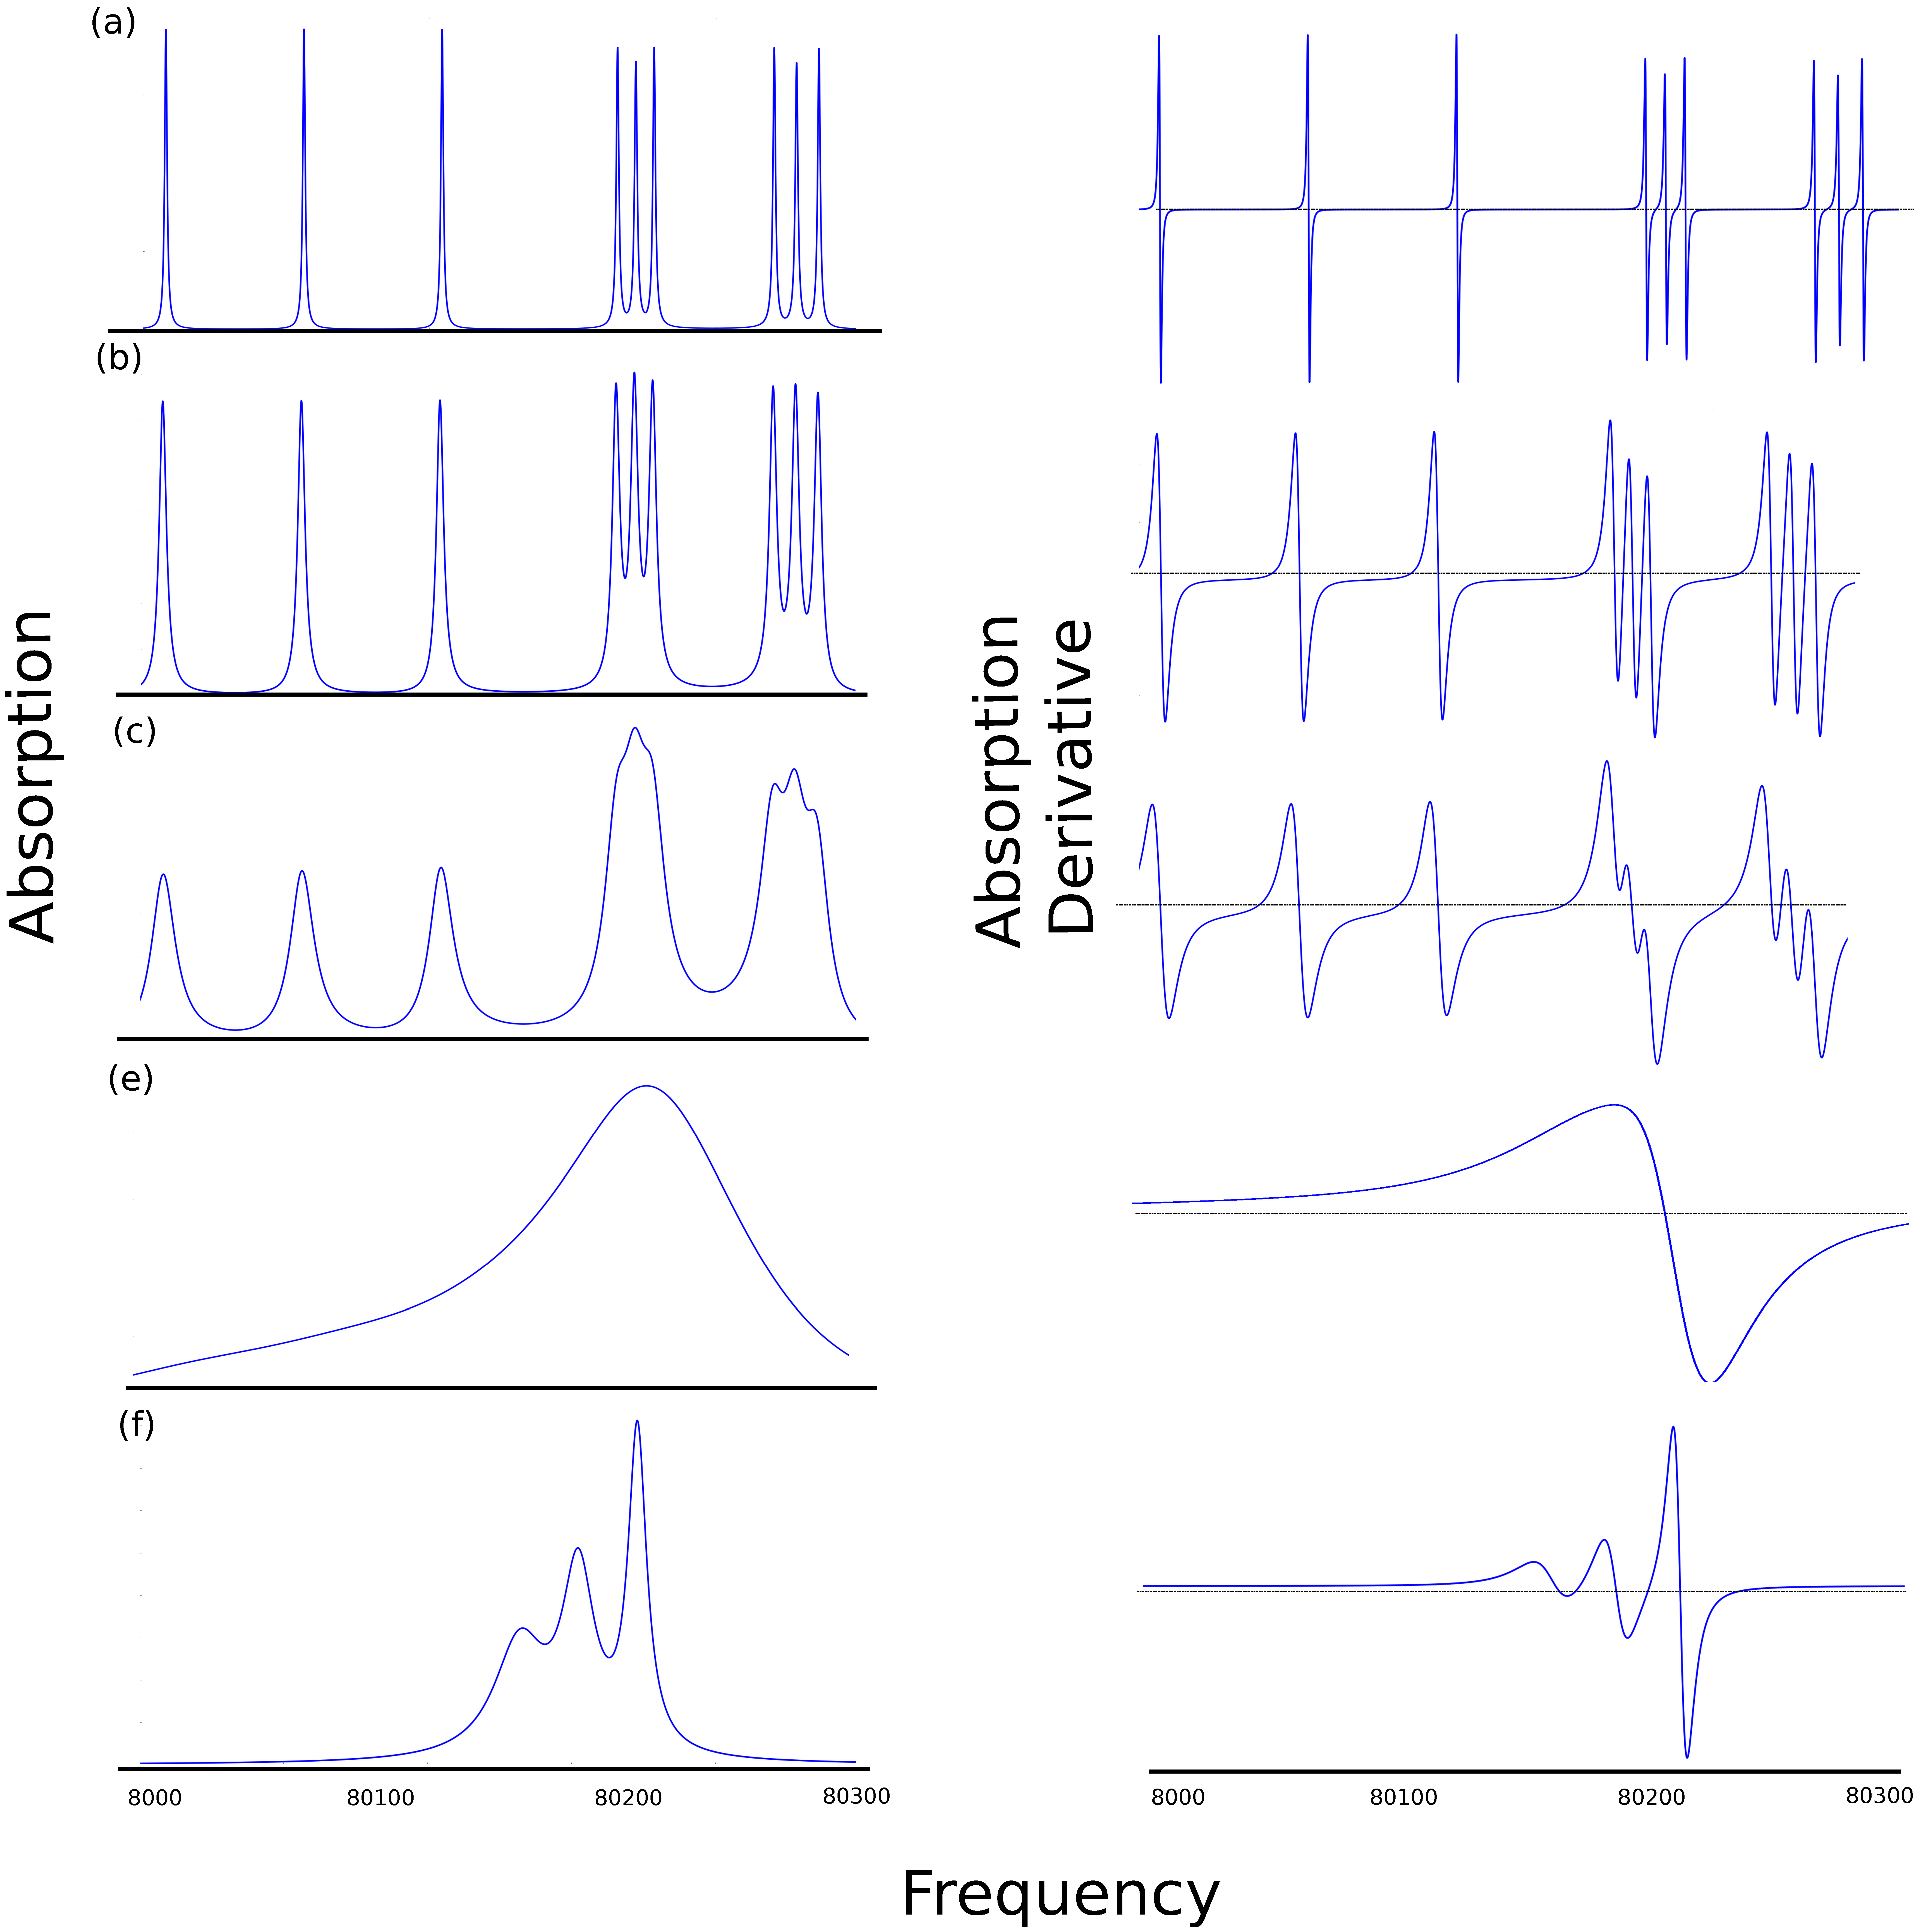
\includegraphics[width=1\textwidth]{figures/chap2/spinone.eps}
\caption{Evolution of NMR line shapes with increase of transition rates $W$ for $I=1/2$ nucleus in a fixed magnetic field along $z$ axis and fluctuating local magnetic fields $h$ along (a) $x$ axis, (b) $y$ axis and (c) $z$ axis. Simulated using AI alagorithm}
\label{figure:spin05der}
\end{figure}
\clearpage